% This a LaTeX template for a research journal, aimed at 
% being 
% 1. easy to use, so one can simply type the daily entries;
% 2. elegant.
% It was written by Níckolas Alves (alves-nickolas.github.io)

% THIS WAS ORIGINALLY COMPILED WITH LUALATEX, so I suggest going to the Menu (top-left of your screen, if you're on Overleaf) and selecting LuaLaTeX on Settings -> Compiler. I didn't test it on XeLaTeX, but I think it should work fine as well. While the document will still compile on pdfLaTeX, for example, it will not have access to the FiraMath font, and hence math text will look weird (it will be typeset in LaTeX's standard Computer Modern Math). If you don't plan on using mathematics at all, then there is a reasonable chance pdfLaTeX will do just fine

\documentclass[a4paper, 11pt, oneside]{researchjournal} % I wrote the design using a4paper, 11pt, oneside, but feel free to change

\usepackage[margin=0.7in]{geometry}
\usepackage{cleveref}
\usepackage{parskip}
\usepackage{tikz}
\usepackage{siunitx}
\usepackage{pgfplots}

%\logo{} can be used to add a small decoration to the top of the cover page. My original idea was to put an \insergraphics command in it and load, e.g., the university logo or something

\author{Siddhant Pujni\\ % you can use double bars to add lines to the author decoration on the main page
The University of Edinburgh}

% colors are customizable using xcolor's (https://ctan.org/pkg/xcolor) \definecolor
\definecolor{ChapterBackground}{HTML}{101010} %colors to use on chapters
\definecolor{ChapterForeground}{HTML}{2FAEA3} %colors to use on chapters
\definecolor{DayColor}{HTML}{2FAEA3} %colors to use on newdays and daybibs
\definecolor{CoverBackground}{HTML}{101010} %cover background
\definecolor{CoverForeground}{HTML}{2FAEA3} %cover letters
\definecolor{LinkColor}{HTML}{2FAEA3} %color for links

\begin{document} % this will automatically generate a simple cover

\newday*{2026-01-15} 
Had the preliminary meeting with Romeel yesterday to get going on the project. Had already contacted and set-up required Python packages and Linux. Was given an article and a paper that is close to the project. They are more observational, and we will be doing something similar, but for the SIMBA simulations. CAESAR takes snapshots of the simulation of all galaxies at a specific redshift and outputs their properties, including absolute magnitude, apparent magnitude, etc. We will meet every Wednesday at 11 am, and I will prepare a small set of slides for these meetings to cover what I have achieved and done over the last week; mostly figures and images, just to refer to for report writing. 

\vspace{0.5em}

The paper discusses \parencite{hillSpectrumUniverse2018}.

\vspace{0.5em}

The article discusses \parencite{bakerWhatColorUniverse2021}.

Need to do more reading regarding and learn about:
\begin{itemize}
\itemsep -6pt {}
    \item CAESAR documentation (specifically Photometry section)
    \item FSPS
    \item H5py for file reading
    \item also set up the GitHub repo for organised work
\end{itemize}

Also assigned the first task, which is to replicate Figure 4 from \parencite{hillSpectrumUniverse2018}, but just for one snapshot of the SIMBA simulation. The goal is to essentially look at all galaxies at some redshift and sum up their fluxes for each band, then plot them by extracting wavelength and magnitudes. Adding up all intensities for each filter and then plotting each filter at its respective frequency.

\newday{2026-01-16}
Goals for the day:
\begin{itemize}
\itemsep -6pt {}
    \item Set up the GitHub repo 
    \item Read necessary documentations
    \item Figure out what exactly the graph is plotting and what $\nu I_{\nu}$ is. 
\end{itemize}

Using the CAESAR Catalogue with 25 Mpc/h volume and $2\times256^3$ particles, at z=0.

Spent some time setting up the GitHub repo with working references from zotero and Overleaf linking for report writing and referencing. Everything now works as one big thing together.

\newday{2026-01-17} Worked on building the SED of all galaxies in all bands from the Caesar catalogue. The catalogue was loaded via caesar.load, and a basic histogram in \cref{fig:mass_diss} of log10(total mass) by extracting each galaxy’s total mass (i.masses['total']) was used to visualise the overall galaxy population. Some time was spent to learn and familiarising with the overall file and data structure of the hdf5 files in general.
 
\begin{figure}[htbp]
    \centering
    \includegraphics[width=0.7\textwidth]{figures/optical/week_1/mass_diss.png}
    \caption{Histogram of total galaxy mass from the SIMBA z=0 snapshot.}
    \label{fig:mass_diss}
\end{figure}

\newpage 

Essentially constructed a catalogue-wide SED from stored apparent magnitudes accounting for dust (galaxy\_data/dicts/appmag.*): for each filter it converts magnitudes to flux density using the AB relation $F_\nu = 3631,\mathrm{Jy},10^{-m/2.5}$, obtains an effective frequency ($\nu$) from the FSPS filter’s effective wavelength $(\nu=c/\lambda_\mathrm{eff})$, sums flux over all galaxies to get a total per-filter $F_\nu$, sorts by frequency, and plots $\nu F_\nu$ versus $\nu$ on log–log axes to show the overall SED shape of the sample across the available bands in \cref{fig:sed_z0}.

\begin{figure}[htbp]
    \centering
    \includegraphics[width=0.7\textwidth]{figures/optical/week_1/galaxy_sed.png}
    \caption{Spectral energy distribution from the SIMBA z=0 snapshot, plotted as $\nu F_{\nu}$ versus frequency $\nu$ (assuming AB magnitudes).}
    \label{fig:sed_z0}
\end{figure}

\newpage

\newday{2026-01-20} Setting up Cuillin login and accessing Simba data through it, needed to learn some linux commands to navigate through directories and files. Managed to access the Simba data and set up a symlink in the home directory to access it for analysis. The goal for the rest of the week is to create the same plot at different redshifts to examine how things evolve over time. Also aiming to break up the SED into different components -- e.g., star-forming galaxies vs quenched galaxies, a range of stellar mass bins to gain a sense of what objects are dominating the overall cosmic light at given wavelengths and redshifts. I need to add more references and papers about the tools that I'm using.

\newday{2026-01-22} Working on looking at the time evolution of full galaxy SED across different redshifts. No galaxies have formed above a redshift of z=? (below file number 019) and its only halos so there is no SED to be made. Also will be ignoring snap 151 from now on which is effectively z=0 because apparent = abs magnitude because its at 0 distance from us.

Created a plot in \cref{fig:time_evo_abs_mag_sed} and \cref{fig:time_evo_app_mag_sed} showing the SED at different redshifts from z~9 to z~0 for both apparent and absolute magnitudes just taking occasional redshift jumps. my general understanding for the absolute magnitude SEDs was that as time goes on (lower redshifts) it increases in intensity because more stars and galaxies form over time contributing to overall light. for the apparent magnitude it was more so that we're observing a lot more flux from closer galaxies so higher intensity and is mainly showcasing the distance effects. As for the overall shape my understanding was its determined by hotter bluer stars which contributes to fluxes at shorter wavelengths and the longer redder wavelengths are dominated by older cooler stars the combination of which will make up the overall SED. Interestingly though in the absolute mags the lowest z are not the very highest curves.  but of course in apparent mags they are farther away so they appear fainter. The general shape also changes with redshift, which has to do with how many older vs younger stars there are.

\begin{figure}[htbp]
    \centering
    \includegraphics[width=0.8\textwidth]{figures/optical/week_2/time_evo_abs_mag_SED.png}
    \caption{Time evolution of the spectral energy distribution of absolute magnitudes from the SIMBA snapshots, plotted as $\nu F_{\nu}$ versus wavelength $\lambda$ (assuming AB magnitudes).}
    \label{fig:time_evo_abs_mag_sed}
\end{figure}

\begin{figure}[hbt!]
    \centering
    \includegraphics[width=0.8\textwidth]{figures/optical/week_2/time_evo_app_mag_SED.png}
    \caption{Time evolution of the spectral energy distribution of apparent magnitudes from the SIMBA snapshots, plotted as $\nu F_{\nu}$ versus wavelength $\lambda$ (assuming AB magnitudes).}
    \label{fig:time_evo_app_mag_sed}
\end{figure}

\newpage

\newday{2026-01-23} Aiming to dive deeper and explore the above graphs by taking one of the redshifts and splitting it into bins of various galaxy types, e.g. star-forming galaxies vs quenched galaxies, different stellar mass bins, etc.
Going to be defining quenched galaxies using SFR (instantaneous), SFR\_100 (avg SFR over last 100My), and sSFR ($\frac{\text{sfr}}{M_*}$, $M_*$ is total galaxy stellar mass).

Below in \cref{fig:abs_mag_mass_bins_sed} the SED is binned by stellar mass and using absolute magnitude, which was done using log(stellar\_mass) into 4 equal bins just so they're all the same ratio in ranges. i wasnt quite sure, but my interpretation of these graphs was that for larger galaxies (higher stellar mass), they were much brighter than low stellar mass, with the number of galaxies in that mass range also playing a role in overall flux. for higher redshifts, the galaxies seem to be significantly bluer, but i thought they'd be redder since older galaxies would have less younger bluer stars and be more IR dominated and redder but maybe the redshift just isn't high enough?
Note: for z>5 there are no galaxies in the largest mass bin- implying that massive galaxies don't exist at those redshifts yet.

\begin{figure}[htbp]
    \centering
    \includegraphics[width=0.6\textwidth]{figures/optical/week_2/abs_mag_stellar_mass_binned_SED.png}
    \caption{Absolute Magnitude SEDs binned by stellar mass at a range of redshifts.}
    \label{fig:abs_mag_mass_bins_sed}
\end{figure}

\begin{figure}[htbp]
    \centering
    \includegraphics[width=0.6\textwidth]{figures/optical/week_2/app_mag_stellar_mass_binned_SED.png}
    \caption{Apparent Magnitude SEDs binned by stellar mass at a range of redshifts.}
    \label{fig:app_mag_mass_bins_sed}
\end{figure}

For plotting quenched galaxies vs star-forming galaxies in \cref{fig:abs_mag_quenched_sed} and \cref{fig:app_mag_quenched_sed}, I used a ssfr threshold of $10^{-11} yr^{-1}$ to define quenched galaxies, which was quoted in literature in \parencite{boselliQuenchingStarFormation2016} on page 17 and also \parencite{wetzelGalaxyEvolutionGroups2012}. My interpretation of these graphs was that the star forming galaxies were significantly brighter than the quenched galaxies across all wavelengths, which made sense since they have a lot more young hot blue stars contributing to the overall flux. The quenched galaxies were also redder, as expected, since they have older, cooler stars dominating their SEDs and the star forming galaxies are much bluer due to the abundance of young hot stars.

\begin{figure}[htbp]
    \centering
    \includegraphics[width=0.6\textwidth]{figures/optical/week_2/abs_mag_quenced_starforming_SED.png}
    \caption{Absolute Magnitude SEDs binned by quenched vs star-forming galaxies at a range of redshifts.}
    \label{fig:abs_mag_quenched_sed}
\end{figure}

\begin{figure}[htbp]
    \centering
    \includegraphics[width=0.6\textwidth]{figures/optical/week_2/app_mag_quenced_starforming_SED.png}
    \caption{Apparent Magnitude SEDs binned by quenched vs star-forming galaxies at a range of redshifts.}
    \label{fig:app_mag_quenched_sed}
\end{figure}

\newpage

\newday{2026-01-27} I think the next thing is to combine these outputs into making a prediction for the observed cosmic SED. This means accounting for the fact that the higher-z ones will be dimmer. The easiest way is probably to make a light cone. Then can just sum up all the apparent magnitudes appropriately to get the total.

\vspace{1em} 

Chris Lovell has made a small code to create lightcones from Simba snapshots:\\ https://github.com/christopherlovell/simba\_lightcone\_generation (\parencite{lovellChristopherSimba_lightcone_generation2021}). Looking at Chris's code it uses hardcoded paths to supercomputer cosma7 and SIMBA run with a 100 Mpc/h volume with 1024 particles. As a result, I have had to kind of repurpose the code to my use case for the run and update it. Main changes made are:

Files 1-9 (above $z = 13$) have no halos, so there's no halo data, need to account for that by setting redshift range from 0 to 13 and then dropping files with higher redshift.

At $z \geq 0.5$, the 1 deg$^2$ survey area is larger than the simulation box (25 Mpc). So the selection mask fails because L - A is negative.

The original code contained hardcoded paths to the COSMA filesystem and assumed the \texttt{m100n1024} file naming convention. I updated these to point to my local Caesar catalogue directory and modified the file naming pattern from \texttt{m100n1024\_\{snap\}.hdf5} to \texttt{m25n256\_\{snap\}.hdf5}. Additionally, I removed the \texttt{sim\_directory} variable, which pointed to the raw simulation snapshots, as my analysis only requires the post-processed Caesar catalogues containing pre-computed galaxy properties.

The original code assumed specific unit conventions from the COSMA setup, using \texttt{Mpccm} (comoving Mpc) for positions. However, I found that the Caesar files I was working with used different unit conventions that were not always recognised by \texttt{astropy}. To address this, I implemented flexible unit handling that attempts multiple approaches:

\begin{verbatim}
try:
    pos = g.pos.to('Mpc').value
except:
    try:
        pos = g.pos.value
    except:
        pos = np.array(g.pos)
\end{verbatim}

Similarly, for the simulation box size, I added logic to detect whether the value was stored in kpc or Mpc and convert accordingly.

During initial testing, I encountered a \texttt{KeyError} indicating that \texttt{'halo\_data'} did not exist in certain files. I found that this error occurred for snapshots 001--009, which correspond to redshifts $z > 13$. At these epochs, the universe had not yet formed sufficient structure for Caesar to identify any halos or galaxies, hence, these snapshots were skipped. The main lightcone generation function then checks for these \texttt{None} returns and skips those snapshots with an informative message.

Finally, I converted the code from a command-line interface using \texttt{argparse} to an importable Python function. This allows for easier integration with the Jupyter notebooks that I am using.

The core lightcone generation algorithm was left the same and works as follows:

\begin{itemize}
\setlength\itemsep{0.5em}
    \item Loops through snapshots sorted by redshift
    \item Selects galaxies within a specified spatial region projected onto RA and DEC
    \item Assigns observed redshifts based on each galaxy's $z$-coordinate combined with the comoving distance to the snapshot
    \item Saves the resulting lightcone to an HDF5 file containing galaxy indices, redshifts, positions, and stellar masses
\end{itemize}

\newday*{2026-01-28} 

What is a lightcone?

A lightcone is a geometric construct that represents the path of light travelling through spacetime from distant sources to an observer. In the context of galaxy surveys and cosmological simulations, a lightcone catalogue mimics what a real telescope would observe: galaxies at different distances are seen at different cosmic times, since light from more distant galaxies has taken longer to reach us. A galaxy observed at redshift $z = 2$, for example, is seen as it was approximately 10 billion years ago, when the universe was younger, denser, and galaxies were typically less massive and more actively star-forming.

Constructing a lightcone from a simulation involves stitching together multiple simulation snapshots, each representing the universe at a specific redshift. Galaxies are selected from each snapshot based on their spatial position within a defined survey area (in angular coordinates RA and DEC) and assigned an observed redshift based on their line-of-sight distance. This approach captures the evolution of the galaxy population across cosmic time within a single catalogue, rather than treating each snapshot as an independent, instantaneous view of the universe.

The resulting lightcone allows us to compute observable quantities such as the integrated cosmic background light. By summing the flux contributions from all galaxies in the lightcone---each appropriately dimmed according to its luminosity distance---we obtain a prediction for the total extragalactic background light (EBL) that would be measured by an observer. This is fundamentally different from summing galaxies at a single redshift, as it properly accounts for the fact that the galaxy population evolves with cosmic time and that more distant galaxies contribute less flux due to the inverse-square law and cosmological dimming.

Not looking into by mid IR is dominated by something known as Polycyclic Aromatic Hydrocarbons (PAHs) which are essentially components of interstellar dust and one of the primary forms of carbon in the universe. 

Next part of the project is to look into the far IR spectrum of the cosmic SED which is mainly just from dust in the ISM. Aiming to do this by modelling the dust as a blackbody by using Plancks Law and fitting a range of different mean temperatures $T$ that best fit observational SEDs for far IR and essentially predicting the mean temperature of dust according to SIMBA. Essentially working backwards and empircally fitting a temperature that gives the most accurate/similar SED to observational papers in the far IR part. CAESAR catalogues \texttt{L\_FIR} which is essentially the total energy per second (luminosity, in erg/s) emitted by dust in a galaxy in the far IR part of the spectrum. 

\begin{equation*}
    \rho(\omega, T)
    =
    \cfrac{\hbar \omega^3}{\pi^2 c^3}
    \frac{1}{\exp\big({\frac{\hbar \omega}{k_BT}} - 1\big)},
\end{equation*}

\begin{figure}[htbp]
    \centering
    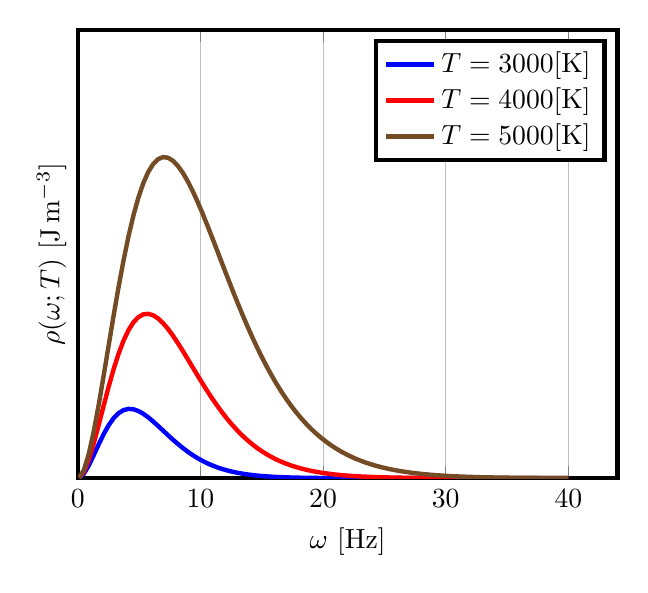
\begin{tikzpicture}[samples=100, scale=1.00]
        \begin{axis}[
            xmin=0,
            xlabel={$\omega$ [\si{\hertz}]},
            ymin=0,
            ymax=pi,
            ylabel={$\rho (\omega; T)$ [\si{\joule\per\cubic\meter}]},
            ytick=\empty,
            no markers,
            grid=both,domain=0.1:40,
            style={ultra thick}]
            \pgfplotsinvokeforeach{3000, 4000, 5000}
    {
            \addplot+
            {(x^3)/((pi^2)*(exp(2000*x/(#1))-1))};
            \addlegendentryexpanded{$T = #1 [\si{\kelvin}]$}
    }
        \end{axis}
    \end{tikzpicture}
    \caption{Blackbody Spectrum for different temperatures.}
    \label{fig:PlancksBlackbodySpectrum}
\end{figure}

% look at cosmic ir spectrum for mid ir

% empircally fit xray pre factor value using the data what the curve should look like and we've got the prefactor that simba says we should have.

% caesar has bucket of far ir energy emissions, lfarir

% spectrum of dust is blackbody defined by temp and luminosity, we dont know temp and need to make assumptions about it 
% - use observations from the paper and try to work backwards to find mean dust temp of the universe and mess around with an input temperature that fits the far ir blackbody curve. and we basically plot using lfarir and then fit different temperatures to match a curve similar to observations. figure out mean temperature of dust in the universe empircally fit by basically just plotting and seeing ok what temperature actually works when trying to plot lfarir

% bin (what) by redshift and compare to the andrews, driver paper

\newpage

\newday{2026-01-29} Setting up the GitHub repo on the cuillin cluster to access larger data files from Simba run instead of having to copy data over. This involved reinstalling everything on my cuillin directory (miniconda, caesar, etc.) and then making the correct environment and dealing with fsps home environment variable. Found a way to access cuillin through vscode which makes editing and running code significantly easier (especially notebooks) however I am having issues with performance and it feels super slow and am spending more time troubleshooting making cuillin and vscode work than writing any actual code. 

Have not yet started any work on making the mid IR spectra.

\newday{2026-01-30} Romeel said one thing is that the sSFR cut you used is quite restrictive and that the typical SFR of the universe (and galaxies at a given $M_\star$) increases out to $z~2$. So I updated galaxy classification function for sSFR cut to be less restrictive by commensurately updating it with age of universe at redshift $z$. It is now sSFR\_quenched($z$) < 0.2 / t\_H($z$), where t\_H is the age of the universe at redshift $z$ \parencite{rodriguezmonteroMergersStarburstsQuenching2019}. In \cref{fig:updated_abs_mag_quenched_sed} and \cref{fig:updated_app_mag_quenched_sed} we see very similar overall shapes and trends, the main difference is just the number of galaxies observed at different redshifts. We're even seeing quenched galaxies at high redshfits now rather than there being no curve.

\begin{figure}[htbp]
    \centering
    \includegraphics[width=0.6\linewidth]{figures/optical/week_3/m25n256/updated_abs_mag_quenched_starforming_SED.png}
    \caption{Updated figure for absolute magnitude with a less restrictive cut to define what a quenched galaxy is considered to be.}
    \label{fig:updated_abs_mag_quenched_sed}
\end{figure}

\begin{figure}[htbp]
    \centering
    \includegraphics[width=0.6\linewidth]{figures/optical/week_3/m25n256/updated_app_mag_quenched_starforming_SED.png}
    \caption{Updated figure for apparent magnitude with a less restrictive cut to define what a quenched galaxy is considered to be.}
    \label{fig:updated_app_mag_quenched_sed}
\end{figure}

\noindent Also have first major result of the project (although only for the smaller m25n256 run). In \cref{fig:optical_range_SED} we can see the flux from all galaxies in the optical part of the spectrum taken using a lightcone giving a rough idea of the optical 'colour' of the universe. Done using Chris Lovell's code and as described earlier.

\begin{figure}[htbp]
    \centering
    \includegraphics[width=0.5\linewidth]{figures/optical/week_3/m25n256/optical_lightcone_SED.png}
    \caption{Final observed Cosmic SED in the Optical/Near IR range.}
    \label{fig:optical_range_SED}
\end{figure}

\noindent In \cref{fig:galaxy_number_lightcone_distribuition} is also a distribution of the number of galaxies at different redshifts found by the lighcone function:

 \begin{figure}[htbp]
     \centering
     \includegraphics[width=0.5\linewidth]{figures/optical/week_3/m25n256/lightcone_redshift_distribuition.png}
     \caption{Number of galaxies at a range of redshifts within the lightcone.}
     \label{fig:galaxy_number_lightcone_distribuition}
 \end{figure}

\newpage

\newday{2026-02-02}

Since dust is not a perfect blackbody and results in spectrums slightly cooler and less efficient at emitting at shorter wavelengths the Planck law seems a bit too simplified and dust is not a great blackbody but more of a 'greybody' which is better fit by a modified blackbody (MBB) which is just the normal Planck Law multiplied by frequency dependent emissivity, typically a power. This term is usually some sort of emissivity function $\epsilon_\nu$ and assumes that the source is optically thin meaning light entering exits without significant absorption ($\tau \ll 1$) \parencite{SubmillimeterGalaxiesAW, MBBFitsInterstellar}. It is of some form:

\begin{equation*}
    f_\nu \propto [1 - \text{exp}(-\tau_\nu)]B_\nu,
\end{equation*}
\noindent where $\tau_\nu$ is the frequency-dependent optical depth of the cloud, and is a multiple of $\epsilon_\nu$.

Also found another recent paper which basically says that a single temp along a line of sight isn't sufficient and basically derives a Gaussian distribution of temps along the line of sight around a central mean temp. what i could do here is assume the temp distribution is centred about some mean T which i vary and test as we were originally going to but we would also need to fit for the width of that distribution i believe which is the dispersion. It uses the first and second derivatives of the Planck function where I know we use the first to find Weins law and google says the second one is the curvature and breadth of the spectrum. I would also need to correct for the CMB radiation which it gives an equation for using radiative transfer. Alternatively the easier (and i think more common approach) is just to use the MBB with a single temperature and range $T$, $\epsilon$ \parencite{desertInterstellarDustEmission2022}.

\newday{2026-02-03}
Romeel found another paper which models $T_\text{dust}$ against various properties using cosmological simulations from FIRE which provides an equation that could be used to predict the dust temperature to feed into the MBB I will use \parencite{liangDustTemperaturesHighredshift2019}. Below I quote equation (15) which is a two parameter fit for $T_\text{eqv}$ with $\delta_\text{dzr}$ and redshift as predictor variables from the paper,

\begin{equation*}
    \log({T_\text{eqv}/25\text{K}) = a + b \log{(\delta_\text{dzr}/0.4)}+ c \log(1+z)},
    \label{eq:equivalentDustTemp}
\end{equation*}

\noindent where a, b, and c are the best fitting regression parameters a range of which are provided in table 2 in the paper. We will be going with band 6 OT-MBB values which is the optically thin modified blackbody and band 6 has a wavelength of $870\mu\text{m}$ which fits the typical range of far IR as band 7 was too high. This seemed like the most reasonable approach as far IR emission is typically from dust in the ISM which is typically assumed to be optically thin. Here $T_\text{eqv}$ is the assumed dust temperature which is conceptually different from $T_\text{eff}$ because the former is an assumed quantity for extrapolating total infrared luminosity, $L_\text{IR}$, from a single data point while the latter is a derived quantity through SED fitting to multiple data points \parencite{liangDustTemperaturesHighredshift2019}. Finally, $\delta_\text{dzr}$ is the dust to metal ratio which can be computed by (dust mass / (metallicity * gas mass)) \cite{liDusttoGasDusttoMetalsRatio2019}.

This does mean the approach for far IR has been slightly altered in the sense that now I will use the temperature formula above directly as if its valid for all $z$ (even though the paper models for $2 \le z \le 6$). I can compute $\delta_\text{dzr}$ for every galaxy from catalogues and $z$ is known which gives a $T_\text{eqv}$ for each galaxy which can then be used in the MBB formula to generate a spectrum for each galaxy, then summed up to find total far IR SED. The value for the dust emissivity spectral index, $\beta$, was inferred from literature to be \~2.

\newday*{2026-02-05}
Was not a super productive week in terms of results, however, I focused more on a literature review on what is currently out there in terms of dust modelling for simulations and planning an approach to build the far IR spectrum. Discussed this with Romeel in the meeting where we ironed out the approach and I verified the assumptions I was making for the modelling of the dust.

We discussed possibly using an MCMC fit to model and fit the best fitting regression parameters a, b, c to see which produces the best spectra. Potentially looking into an MCMC for $T_{eqv}$ and $\beta$ if the current approach does not work out fully. 

\newday{2026-02-08}
Began by researching into the MBB and what the equation would look like. The MBB spectral energy distribution per unit wavelength is given by:

\begin{equation}
    S_\lambda(\lambda, T) = N \left( \frac{\lambda}{100\,\mu\mathrm{m}} \right)^\beta \frac{2 h c^2}{\lambda^5} \frac{1}{\exp\left(\frac{h c}{\lambda k_B T}\right) - 1},
    \label{eq:mbb}
\end{equation}
\noindent where $\lambda$ is the wavelength, $T$ is the dust temperature, $\beta$ is the dust emissivity index, $N$ is a normalisation constant, $h$ is Planck's constant, $c$ is the speed of light, and $k_B$ is Boltzmann's constant.

Furthermore, to ensure the total far-infrared luminosity ($L_\mathrm{FIR}$) matches observations or model constraints, the MBB is normalised such that:

\begin{equation}
    \int S_\lambda(\lambda, T)\, d\lambda = L_\mathrm{FIR}
\end{equation}

This is achieved by computing the integral of the unnormalised SED and scaling the spectrum so its total energy output equals $L_\mathrm{FIR}$. This step was necessary to connect the theoretical SED shape to the observed or desired luminosity, ensuring physical consistency.

This is the basic set-up for building the SED but right now the code computes for each individual galaxy and then sums all galaxies in a singular snapshot. However, similar to the optical SED, a lightcone will need to be used to generate the final SED to capture the effect over time/redshift. 

\newday{2026-02-10}

While working on the code over the last few days I have realised that at this point using Jupyter Notebooks was not optimal since it wasn't running through the IFA cluster, and it was very manual in regards to what SIMBA run was being used. So I spent the entire day refactoring the GitHub repository to take user input with which SIMBA run was being used, the choice of generating an SED for optical or far IR, and transferring all primary functions into .py files rather than floating around in notebooks. The repo feels much more professional now and code is running much quicker.

\newday*{2026-02-11} Meeting day but Romeel was travelling and we did not meet. Taking the time to debug the far IR code as there were a few issues. The first was there was a lot of nan values in $T_{eqv}$ and $\delta_{dzr}$ that were throwing errors with the code as it would not run, just added some handling to ignore any nan or close to zero values that show in order to avoid division by zero errors. Secondly, although caesar computes $L_\mathrm{FIR}$ when photometry is done, this was not always done in every single snap, as a result, when going through some snaps this would lead to hdf5 not being able to access any $L_\mathrm{FIR}$ values and crashing. These snaps were random and not ones on the edge cases of redshift so some more handling was added to skip snaps where a $L_\mathrm{FIR}$ could not be accessed. This has likely led to some lost data, however, it won't be a significant amount due to the volume of the snaps and data we have. Finally, after these were dealt with the SED being produced does not have anywhere near the expected shape of a curve. Overall the code and primary logic for generating the spectrum is now complete as we are summing the total flux using the lightcone but the graph is not as expected and has sharp edges (very sorry I thought I had saved it but am realising its gone). 

Did realise I can use the same lightcone for both optical and far IR it just needs to be processed differently. This will speed things up (especially for the m100n1024 run) as I only need to generate the lightcone for the necessary run, area, and redshift range once.

\newday{2026-02-12} Progress has felt slow over the last week as I have been spending a lot of time on TGP so have not been able to focus here as much as I would like. However, I believe the final SED for the far IR range is ready now and I have sent my results to Romeel just waiting on a response and next steps. I am also not sure what the approach for the MCMC fitting of best fit parameters is as I don't actually have any observed data, but the code itself is easy enough to write with \texttt{emcee} when it comes to it.

Finally, the issue with the code was that instead of using $\log_{10}$ I was using $\ln$ in \cref{eq:equivalentDustTemp} as that's what \texttt{np.log()} defaults to and there was also a sign error in the formula. After fixing these issues I was able to produce a SED that was roughly as per expectations. Below I present 6 graphs for each SIMBA run for both optical and far IR SED

\begin{figure}[htbp]
    \centering
    \includegraphics[width=0.6\textwidth]{figures/optical/optical_bg_m25n256.png}
    \caption{Final optical/near IR SED from SIMBA simulation for the 25 Mpc/h box with $256^3$ dark matter and $256^3$ gas elements.}
    \label{fig:optical_bg_m25n256}
\end{figure}

\begin{figure}[htbp]
    \centering
    \includegraphics[width=0.6\textwidth]{figures/optical/optical_bg_m50n512.png}
    \caption{Final optical/near IR SED from SIMBA simulation for the 50 Mpc/h box with $512^3$ dark matter and $512^3$ gas elements.}
    \label{fig:optical_bg_m50n512}
\end{figure}

\begin{figure}[htbp]
    \centering
    \includegraphics[width=0.6\textwidth]{figures/optical/optical_bg_m100n1024.png}
    \caption{Final optical/near IR SED from SIMBA simulation for the 100 Mpc/h box with $1024^3$ dark matter and $1024^3$ gas elements.}
    \label{fig:optical_bg_m100n1024}
\end{figure}

\begin{figure}[htbp]
    \centering
    \includegraphics[width=0.6\textwidth]{figures/farIR/farIR_bg_m25n256.png}
    \caption{Final Far IR SED from SIMBA simulation for the 25 Mpc/h box with $256^3$ dark matter and $256^3$ gas elements.}
    \label{fig:farIR_bg_m25n256}
\end{figure}

\begin{figure}[htbp]
    \centering
    \includegraphics[width=0.6\textwidth]{figures/farIR/farIR_bg_m50n512.png}
    \caption{Final Far IR SED from SIMBA simulation for the 50 Mpc/h box with $512^3$ dark matter and $512^3$ gas elements.}
    \label{fig:farIR_bg_50n512}
\end{figure}

\begin{figure}[htbp]
    \centering
    \includegraphics[width=0.6\textwidth]{figures/farIR/farIR_bg_m100n1024.png}
    \caption{Final Far IR SED from SIMBA simulation for the 100 Mpc/h box with $1024^3$ dark matter and $1024^3$ gas elements.}
    \label{fig:farIR_bg_m100n1024}
\end{figure}

Very minimal differences between the different runs. NEED TO ADD INTERPRETATIONS AND TAKEAWAYS FROM THESE GRAPHS.

Below I also show a graph from Simon Driver that is soon to be published (with a draft paper soon) which compares the SED of different simulations, the most relevant to SIMBA are EAGLE (Baes et al 2018) and the SHARK semi-analytic model (Lagos et al 2019). Our graphs do match up well.

\begin{figure}
    \centering
    \includegraphics[width=0.5\linewidth]{figures/literature/eblallmodels.png}
    \caption{Total SED across the entire wavelength spectrum for different simulations.}
    \label{fig:driverSimulationComparison}
\end{figure}

%realised the teqv formula was wrong had written - instead of + and that my logs were base and i was converting using base e and so stuff was way off

%needed to add handling for optical to run through terminal too not only farIR

%added folder sorting for generated lightcone they going to the wrong spot

%just need to double check that the lightcone generation is working for the optical case, and then we can run it for all sims and make a nice plot. basically what was the logic for skipping snaps cause initially the 25mpc was too small so using 50mpc volume allows some more room to play with and less restrictive cut in general

\end{document}

\daybib\parencite{weinberg1995Foundations,weinberg1996ModernApplications}. %daybib adds the text "References: " underneath the entry. It just prints text without doing anything fancy. I use it to list references that I used on some given day, but didn't make it to the main paragraph. Notice I manually added a period at the end of the line.

\newday{2023-03-03} References are dealt with using \verb|biblatex|. You can add your own my modifying the file \verb|bib.bib|.
